%%%%%%%%%%%%%%%%%%%%%%%%%%%%%%%%%%%%%%%%%%%%%%%%%%%%%%%%%%%%%%%%%%%%%%%%%%%%%%%%
%2345678901234567890123456789012345678901234567890123456789012345678901234567890
%        1         2         3         4         5         6         7         8

\documentclass[letterpaper, 10 pt, conference]{ieeeconf}  % Comment this line out if you need a4paper

%\documentclass[a4paper, 10pt, conference]{ieeeconf}      % Use this line for a4 paper

\IEEEoverridecommandlockouts                              % This command is only needed if 
                                                          % you want to use the \thanks command

\overrideIEEEmargins                                      % Needed to meet printer requirements.

%In case you encounter the following error:
%Error 1010 The PDF file may be corrupt (unable to open PDF file) OR
%Error 1000 An error occurred while parsing a contents stream. Unable to analyze the PDF file.
%This is a known problem with pdfLaTeX conversion filter. The file cannot be opened with acrobat reader
%Please use one of the alternatives below to circumvent this error by uncommenting one or the other
%\pdfobjcompresslevel=0
%\pdfminorversion=4

% See the \addtolength command later in the file to balance the column lengths
% on the last page of the document

% The following packages can be found on http:\\www.ctan.org
\makeatletter
\let\NAT@parse\undefined  % ieeeconf.cls defines a fake \NAT@parse; clear it for natbib
\makeatother
\usepackage[numbers]{natbib}
\usepackage{graphicx}
\usepackage{amsmath,amssymb}
\usepackage{tikz}
\usetikzlibrary{patterns,arrows.meta,calc,shapes.misc}
\usepackage{algorithm}
\usepackage{algpseudocode}
%\usepackage{graphics} % for pdf, bitmapped graphics files
%\usepackage{epsfig} % for postscript graphics files
%\usepackage{mathptmx} % assumes new font selection scheme installed
%\usepackage{times} % assumes new font selection scheme installed
%\usepackage{amsmath} % assumes amsmath package installed
%\usepackage{amssymb}  % assumes amsmath package installed

\newcommand{\solver}{DiSMech Newton}

\title{\LARGE \bf
MAE 263F Project Proposal: \solver
}

\author{Ryan Chaiyakul$^{1}$% <-this % stops a space
\thanks{$^{1}$Department of Mechanical and Aerospace Engineering,
        University of California, Los Angeles, CA 90095, USA
        {\tt\small ryanchaiyakul@ucla.edu}}%
}


\begin{document}



\maketitle
\thispagestyle{empty}
\pagestyle{empty}


%%%%%%%%%%%%%%%%%%%%%%%%%%%%%%%%%%%%%%%%%%%%%%%%%%%%%%%%%%%%%%%%%%%%%%%%%%%%%%%%
\begin{abstract}
We propose \solver, a discrete differential geometry (DDG)-based solver for rods and shells built within the GPU-native Newton physics ecosystem.
We will validate \solver{} and Newton's existing Vertex Block Descent (VBD) solver against analytical theory and experimentally derived laws, compare both solvers qualitatively on Newton's existing examples, and demonstrate soft--fluid coupling with \solver{}.
\end{abstract}

\section{Introduction}

Simulation based on discrete differential geometry (DDG) has been highly successful for deformable linear objects \cite{bergou2008der,bergou2010dvt} and thin shells \cite{grinspun2003des}, and modern implementations \cite{tekinalp2024pyelastica, choi2024dismech, lahoti2025pydismech, lahoti2026matdismech, stolzle2026soromox} have added modular external forces, actuation, and differentiability.
However, these implementations have largely been developed in isolation, with minimal coupling to robotics simulators \cite{todorov2012mujoco, gao2026nvidia} or to solvers for other physical domains such as the material point method (MPM) and smoothed particle hydrodynamics (SPH) \cite{monaghan1992sph}.
As a result, many DDG-based robotics contributions \cite{chen2024deform, chen2025deft} rely on ad hoc implementations tailored to their specific needs, which has limited the adoption of DDG simulators in mainstream robotics research.

Newton \cite{nvidia2025newton}, developed in collaboration with many industry partners, emphasizes a GPU-native, multiphysics-coupled ecosystem.
This makes it an opportune time to build a general-purpose DDG solver that the broader community can use to address shortcomings in existing solvers.
Deformable bodies in such frameworks are typically simulated with extended position-based dynamics (XPBD) \cite{macklin2016xpbd} or Vertex Block Descent (VBD) \cite{chen2024vertex}.
Both methods minimize global solves in favor of local parallelism for GPU performance, which works well for volumetric deformable objects.
However, because these methods update vertices locally, long-range forces in slender rods and thin shells must propagate across many vertices.
Such problems therefore require many iterations to converge, and unconverged solutions exhibit unphysical softening.

We propose to develop \solver, a DDG-based solver within the Newton ecosystem.
We focus on fair comparisons with existing Newton solvers in order to recommend when each should be used, and we explore how DDG-based solvers can be coupled to other physical domains.
We will accomplish this in three phases:

\begin{enumerate}
    \item \textbf{Comparison with theory.} Validate \solver{} and VBD against Euler--Bernoulli theory for rod and shell cantilever beams, and evaluate self-contact and friction against experimentally derived laws for overhand knots \cite{jawed2015knots} and plectonemes \cite{clauvelin2009plectoneme}.
    \item \textbf{Qualitative benchmarks.} Compare \solver{} and VBD on Newton's provided cable, cloth, and multiphysics examples.
    \item \textbf{Fluid coupling.} Demonstrate two-way coupling between \solver{} and SPH, and compare the results against low-Reynolds-number resistive force theory (RFT) \cite{gray1955rft}.
\end{enumerate}

\begin{figure}[t]
    \centering
    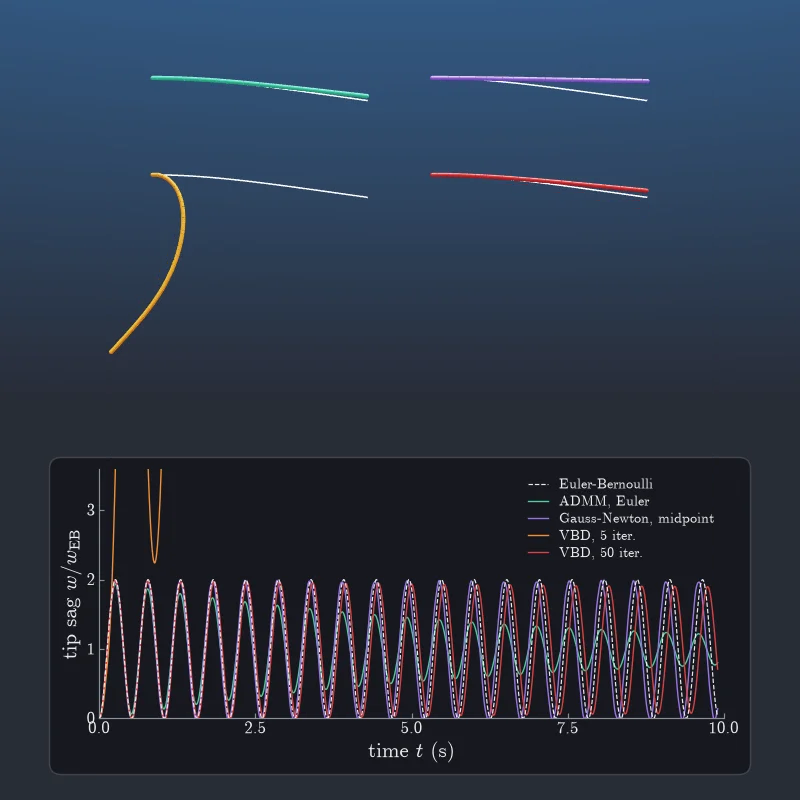
\includegraphics[width=0.9\columnwidth]{teaser.png}
    \caption{Cantilever rod under gravity. \solver{} with ADMM (green) and Gauss--Newton (purple) against Newton's VBD with 5 (orange) and 50 (red) iterations; white lines are the Euler--Bernoulli deflection. Under-iterated VBD softens and diverges.}
    \label{fig:teaser}
\end{figure}

\section{Model}

We model rods with discrete elastic rods (DER) \cite{bergou2008der,bergou2010dvt} and shells with midedge discrete shells \cite{grinspun2003des,chen2018midedge}, as in DiSMech \cite{choi2024dismech} (Fig.~\ref{fig:model}).

\textbf{Degrees of freedom.} A rod with $N$ nodes has DOFs $\mathbf{q} = [\mathbf{x}_0, \theta^0, \mathbf{x}_1, \dots, \mathbf{x}_{N-1}]$, $4N-1$ in total. A shell has three DOFs per vertex and one midedge angle per edge. All bodies share one global vector $\mathbf{q}$ with lumped mass matrix $\mathbf{M}$.

\begin{figure}[t]
    \centering
    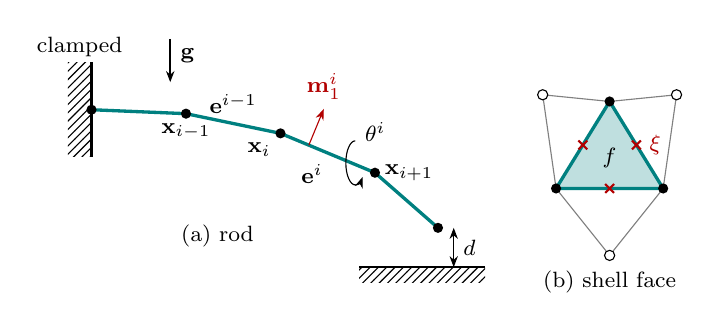
\begin{tikzpicture}[
        node/.style={circle, fill=black, inner sep=1.3pt},
        lbl/.style={font=\footnotesize},
        >={Stealth[length=4pt]}]
        % (a) rod
        \fill[pattern=north east lines] (-0.3,-0.6) rectangle (0,0.6);
        \draw[thick] (0,-0.6) -- (0,0.6);
        \node[lbl] at (-0.15,0.8) {clamped};
        \coordinate (x0) at (0,0);
        \coordinate (x1) at (1.2,-0.05);
        \coordinate (x2) at (2.4,-0.3);
        \coordinate (x3) at (3.6,-0.8);
        \coordinate (x4) at (4.4,-1.5);
        \draw[very thick, teal] (x0) -- (x1) -- (x2) -- (x3) -- (x4);
        \foreach \p in {x0,x1,x2,x3,x4} \node[node] at (\p) {};
        \node[lbl, below] at (x1) {$\mathbf{x}_{i-1}$};
        \node[lbl, below left] at (x2) {$\mathbf{x}_{i}$};
        \node[lbl, right] at (x3) {$\mathbf{x}_{i+1}$};
        \node[lbl, above] at ($(x1)!0.5!(x2)$) {$\mathbf{e}^{i-1}$};
        \node[lbl, below left] at ($(x2)!0.55!(x3)$) {$\mathbf{e}^{i}$};
        % material frame and twist on edge i
        \coordinate (m) at ($(x2)!0.3!(x3)$);
        \draw[->, red!70!black] (m) -- ++(0.19,0.46) node[lbl, above] {$\mathbf{m}_1^i$};
        \draw[->] ($(x2)!0.75!(x3)+(0.05,0.28)$) arc[start angle=90, end angle=320, x radius=0.12, y radius=0.28];
        \node[lbl, above right] at ($(x2)!0.75!(x3)+(0.05,0.15)$) {$\theta^i$};
        % gravity
        \draw[->, thick] (1.0,0.9) -- (1.0,0.35) node[lbl, right, pos=0.4] {$\mathbf{g}$};
        % ground and contact gap
        \fill[pattern=north east lines] (3.4,-2.2) rectangle (5.0,-2.0);
        \draw[thick] (3.4,-2.0) -- (5.0,-2.0);
        \draw[<->] (4.6,-1.5) -- (4.6,-2.0) node[lbl, right, pos=0.5] {$d$};
        \node[lbl] at (1.6,-1.6) {(a) rod};
        % (b) shell face
        \begin{scope}[xshift=5.9cm, yshift=-1.0cm, scale=0.85]
            \coordinate (a) at (0,0); \coordinate (b) at (1.6,0); \coordinate (c) at (0.8,1.3);
            \coordinate (fa) at (1.8,1.4); \coordinate (fb) at (-0.2,1.4); \coordinate (fc) at (0.8,-1.0);
            \draw[gray] (b) -- (fa) -- (c) -- (fb) -- (a) -- (fc) -- (b);
            \fill[teal!25] (a) -- (b) -- (c) -- cycle;
            \draw[very thick, teal] (a) -- (b) -- (c) -- cycle;
            \foreach \p in {a,b,c} \node[node] at (\p) {};
            \foreach \p in {fa,fb,fc} \node[circle, draw, fill=white, inner sep=1.3pt] at (\p) {};
            \foreach \u/\v in {b/c, c/a, a/b} \node[cross out, draw, red!70!black, inner sep=1.2pt, thick] at ($(\u)!0.5!(\v)$) {};
            \node[lbl, red!70!black, right] at ($(b)!0.5!(c)+(0.05,0)$) {$\xi$};
            \node[lbl] at (0.8,0.45) {$f$};
            \node[lbl] at (0.8,-1.4) {(b) shell face};
        \end{scope}
    \end{tikzpicture}
    \caption{Degrees of freedom. (a) A discrete elastic rod: node positions $\mathbf{x}_i$ and edge twist angles $\theta^i$ about the material frame. (b) A midedge shell face $f$: its vertices, the flap vertices across its edges (open), and an angle $\xi$ per edge. Contact acts on gaps $d$.}
    \label{fig:model}
\end{figure}

\textbf{Energies.} The elastic energy is a sum of quadratic penalties on discrete strains $\boldsymbol{\epsilon}(\mathbf{q})$ about their rest values,
\begin{equation}
    E_\text{el}(\mathbf{q}) = \sum_{e} \tfrac{1}{2}\big(\boldsymbol{\epsilon}_e(\mathbf{q}) - \bar{\boldsymbol{\epsilon}}_e\big)^{\!\top} \mathbf{K}_e \big(\boldsymbol{\epsilon}_e(\mathbf{q}) - \bar{\boldsymbol{\epsilon}}_e\big),
\end{equation}
where a rod element (two consecutive edges) has stretching, bending, and twisting strains, and a shell face has membrane (first fundamental form) and bending (second fundamental form) strains.

\textbf{Forces and boundary conditions.} External forces $\mathbf{F}$ include gravity and, for fluid coupling, drag. Contact and Coulomb friction with rigid shapes, other bodies, and self-contact enter as a barrier energy $E_\text{c}(\mathbf{q})$ on the gap $d$ of each contact pair. Clamped boundaries fix a subset of DOFs to prescribed values.

\section{Algorithm}

Each time step of size $h$ solves implicit Euler as a minimization,
\begin{equation}
    \mathbf{q}_{n+1} = \arg\min_{\mathbf{q}} \tfrac{1}{2h^2}\|\mathbf{q} - \tilde{\mathbf{q}}\|^2_\mathbf{M} + E_\text{el}(\mathbf{q}) + E_\text{c}(\mathbf{q}) - \mathbf{F}^\top\mathbf{q},
    \label{eq:ip}
\end{equation}
with prediction $\tilde{\mathbf{q}} = \mathbf{q}_n + h\mathbf{v}_n$.
Following \cite{daviet2023admm}, we split $E_\text{el}$ in strain space with ADMM: each element projects its strains locally in closed form, and the global step solves a linear system whose matrix $\mathbf{A}$ changes only with contact.
Unlike VBD, every iteration is a global solve, so forces propagate along the whole rod in one step (Algorithm~\ref{alg:step}).

\begin{algorithm}[t]
    \caption{\solver{} time step}
    \label{alg:step}
    \begin{algorithmic}[1]
        \Require $\mathbf{q}_n$, $\mathbf{v}_n$, $h$, iterations $K$
        \State $\tilde{\mathbf{q}} \gets \mathbf{q}_n + h\mathbf{v}_n$; $\mathbf{q} \gets \tilde{\mathbf{q}}$ \Comment{predict}
        \State Detect contact pairs; assemble and factor $\mathbf{A}$
        \For{$k = 1, \dots, K$}
            \ForAll{elements $e$ \textbf{in parallel}} \Comment{local}
                \State $\mathbf{z}_e \gets \operatorname{prox}_{E_e}\!\big(\boldsymbol{\epsilon}_e(\mathbf{q}) + \mathbf{u}_e\big)$
                \State $\mathbf{u}_e \gets \mathbf{u}_e + \boldsymbol{\epsilon}_e(\mathbf{q}) - \mathbf{z}_e$
            \EndFor
            \State $\Delta\mathbf{q} \gets -\mathbf{A}^{-1}\nabla\Phi(\mathbf{q})$ \Comment{global}
            \State $\alpha \gets$ line search, capped before first impact
            \State $\mathbf{q} \gets \mathbf{q} + \alpha\Delta\mathbf{q}$
            \If{a node moved past half its radius}
                \State Re-detect contact pairs
            \EndIf
            \If{converged} \textbf{break} \EndIf
            \State Update friction and contact multipliers
        \EndFor
        \State $\mathbf{q}_{n+1} \gets \mathbf{q}$; $\mathbf{v}_{n+1} \gets (\mathbf{q}_{n+1} - \mathbf{q}_n)/h$
    \end{algorithmic}
\end{algorithm}

Here $\Phi$ is the objective of \eqref{eq:ip} with $E_\text{el}$ replaced by its ADMM penalty $\sum_e \tfrac{1}{2}\|\boldsymbol{\epsilon}_e(\mathbf{q}) - \mathbf{z}_e + \mathbf{u}_e\|^2_{\mathbf{P}_e}$.
For validation we also run an exact Gauss--Newton variant that refactors $\mathbf{A}$ at every iterate.


\addtolength{\textheight}{-12cm}   % This command serves to balance the column lengths
                                  % on the last page of the document manually. It shortens
                                  % the textheight of the last page by a suitable amount.
                                  % This command does not take effect until the next page
                                  % so it should come on the page before the last. Make
                                  % sure that you do not shorten the textheight too much.

%%%%%%%%%%%%%%%%%%%%%%%%%%%%%%%%%%%%%%%%%%%%%%%%%%%%%%%%%%%%%%%%%%%%%%%%%%%%%%%%
\bibliographystyle{IEEEtran}
\bibliography{proposal}

%%%%%%%%%%%%%%%%%%%%%%%%%%%%%%%%%%%%%%%%%%%%%%%%%%%%%%%%%%%%%%%%%%%%%%%%%%%%%%%%



%%%%%%%%%%%%%%%%%%%%%%%%%%%%%%%%%%%%%%%%%%%%%%%%%%%%%%%%%%%%%%%%%%%%%%%%%%%%%%%%
\section*{APPENDIX}


%%%%%%%%%%%%%%%%%%%%%%%%%%%%%%%%%%%%%%%%%%%%%%%%%%%%%%%%%%%%%%%%%%%%%%%%%%%%%%%%

\end{document}
